\section{Analog to digital conversion}
The analog to digital conversion aims at reading the luminance of the room, sending the sample to microcontroller. The input channel is feed by the voltage passing through a photoresistor. After having measured that voltage in condition of both full and absence of light, the dynamics has approximated at range [0.5 - 3.0] Volt.
\newline
The chip is ultra-small, low-Power, 16-Bit analog-to-digital converter with internal reference, provided by Texas Instrument at 3.50\$.
The microcontroller drives it by means of an I2C interface.
\begin{figure}[H]
\centering
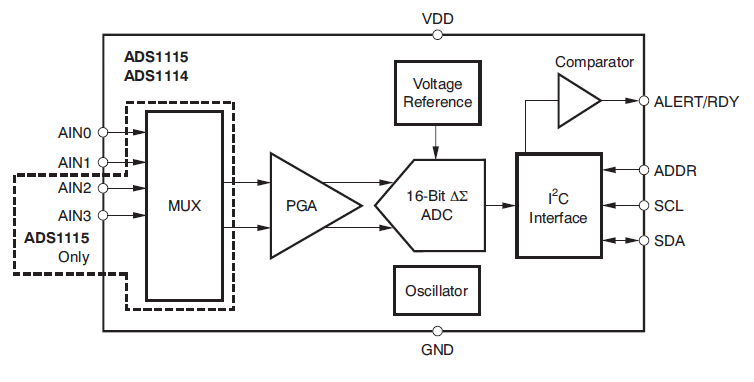
\includegraphics[scale=.7]{Immagini/06}
\label{06}
\caption{A2D internal architecture, from datasheet}
\end{figure}
The chip operates either in continuous conversion mode or a single-shot mode that automatically powers down after a conversion and greatly reduces current consumption during idle periods. I decided to work in the single shot one, sending the command directly from the microcontroller. 
\newline
\newline
In general, to write and read 4 bytes must be sent, the string is composed of the \textbf{slave address} (0x48), the \textbf{register address}, and then in the big-endian format 2 bytes of data. Due to the fact I choose to operate in single shot mode, I have to send every time the command, so the protocol gets as follows: write 4 bytes (including the command), write the slave address and the register address containing the converted data and read 2 byte from it.
\begin{table}[H]
\centering
\begin{tabular}{p{0.5\textwidth}p{0.4\textwidth}}

\textbf{Bit(s) name}&\textbf{Description}\\ \hline
Command & Begin conversion (automatically cleared when completed) \\ 
Input multiplexer configuration & Channel P: In0, Channel N: In1 (physically grounded on breadboard)\\ 
Programmable gain amplifier configuration & $\pm 2.048V$\\
Device operating mode & Power-down single shot mode\\
Data rate & 8 sample per second \\
Comparator mode & not used \\
Comparator polarity & not used \\
Latching comparator & not used \\ \hline
\end{tabular}
\caption{A2D configuration}
\end{table}

\begin{figure}[H]
\centering
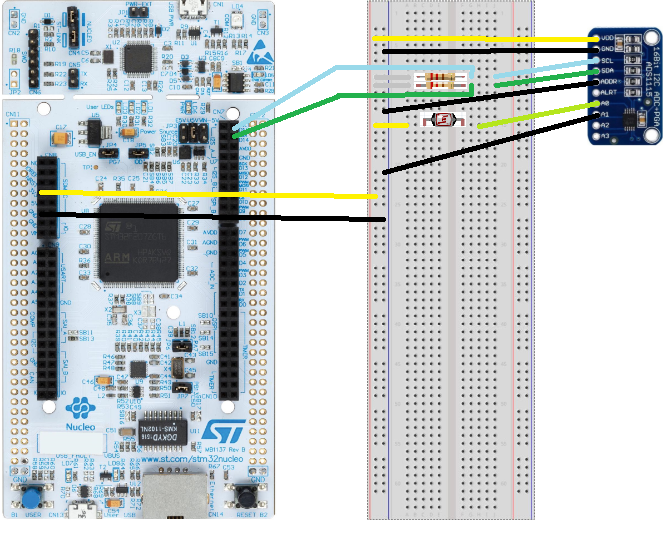
\includegraphics{Immagini/07}
\label{07}
\caption{Connection between MCU and A2D}
\end{figure}

\begin{table}[H]
\centering
\begin{tabular}{p{0.2\textwidth}p{0.4\textwidth}p{0.2\textwidth}}

\textbf{GPIO}&\textbf{Morpho Connector}&\textbf{Description}\\ \hline
PB8 & D15 & I2C1\_SCL\\ 
PB9 & D14 & I2C1\_SDA\\ 
\hline
\end{tabular}
\caption{A2D: GPIOs involved}
\end{table}
